%%%%%%%%%%%%%%%%%%%%%%%%%%%%%%%%%%%%%%%%%%%%%%%%%%%%%%%%%%%%%%%%%%%%%%%%%%%%%%%%%%
\begin{frame}[fragile]\frametitle{}
\begin{center}
{\Large Inferential Statistics}
\end{center}
\end{frame}

%%%%%%%%%%%%%%%%%%%%%%%%%%%%%%%%%%%%%%%%%%%%%%%%%%%%%%%%%%%
\begin{frame}[fragile]\frametitle{What is Inferential Statistics?}
{\bf Inferring} from whats not fully available.
\begin{itemize}
\item Discover properties of larger group by studying smaller group, with a quantified confidence that results generalize well with the larger group.
\item There is a chance (here comes Probability) that sample's behavior can be similar to Population's.
\item Used to compare variables/groups
\end{itemize}
\end{frame}

%%%%%%%%%%%%%%%%%%%%%%%%%%%%%%%%%%%%%%%%%%%%%%%%%%%%%%%%%%%%
%\begin{frame}[fragile]\frametitle{Questions asked in Inferential Statistics}
%\begin{center}
%\includegraphics[width=0.4\linewidth,keepaspectratio]{da1}
%\end{center}
%\begin{itemize}
%\item How does your class compare with other 5th grade classes in the school?
%\item In the district? state?
%\end{itemize}
%\end{frame}


%%%%%%%%%%%%%%%%%%%%%%%%%%%%%%%%%%%%%%%%%%%%%%%%%%%%%%%%%%%
\begin{frame}[fragile]\frametitle{Inferential Statistics Objectives}
\begin{itemize}
\item To estimate, predict a population `parameter' using sample value (called `statistic')
\item Eg Predicting election results based of Exit Polls.
\item Test Hypotheses. 
\item E.g. Whether the new method realy works or not.
\end{itemize}
\end{frame}

%%%%%%%%%%%%%%%%%%%%%%%%%%%%%%%%%%%%%%%%%%%%%%%%%%%%%%%%%%%
\begin{frame}[fragile]\frametitle{Estimate/Predict Population Parameter}
\begin{itemize}
\item Population: Big/Whole dataset
\item Sample: Small/test dataset
\item Point Estimate: using a single value of sample (called `statistic') to predict corresponding value in the population (called `parameter')
\item E.g. Mean of sample can very well be used to estimate Population mean.
%\item Confidence Interval to estimate Population mean
\end{itemize}
\end{frame}


%%%%%%%%%%%%%%%%%%%%%%%%%%%%%%%%%%%%%%%%%%%%%%%%%%%%%%%%%%%
\begin{frame}[fragile]\frametitle{Test Hypothesis}
\begin{itemize}
\item Types: Null Hypothesis ($H_0$) and Alternate Hypothesis ($H_1$)
\item Null Hypothesis: two groups under study are same
\item Alternate Hypothesis: two groups are different
\item Goal: to prove Null Hypothesis wrong
\end{itemize}
\end{frame}

%%%%%%%%%%%%%%%%%%%%%%%%%%%%%%%%%%%%%%%%%%%%%%%%%%%%%%%%%%%
\begin{frame}[fragile]\frametitle{Inferential Statistics Types}
Based on type of distribution:
\begin{itemize}
\item Parametric: Variable is assumed normally distributed
\item NonParametric: Distribution of scores is severely skewed
\end{itemize}
\end{frame}

%%%%%%%%%%%%%%%%%%%%%%%%%%%%%%%%%%%%%%%%%%%%%%%%%%%%%%%%%%%
\begin{frame}[fragile]\frametitle{Inferential Statistics Types}
Based on type of underlying variable:
\begin{itemize}
\item For nominal variables: compare distributions, central tendencies, measure spreads
\item For ordinal variables: non-parametric tests, rank order differences
\item Continuous: Ratio or Interval variables: regression analysis
\end{itemize}
\end{frame}


%%%%%%%%%%%%%%%%%%%%%%%%%%%%%%%%%%%%%%%%%%%%%%%%%%%%%%%%%%%%%%%%%%%%%%%%%%%%%%%%%%
\begin{frame}[fragile]\frametitle{}

\begin{center}
{\large Some Statistical Terms}
\end{center}
\end{frame}


%%%%%%%%%%%%%%%%%%%%%%%%%%%%%%%%%%%%%%%%%%%%%%%%%%%%%%%%%%
\begin{frame}[fragile]\frametitle{Z-score}
\begin{itemize}
\item Meaning: number of std deviations a value is from the mean
\item Example:
	\begin{itemize}
	\item $\mu = 540$
	\item $\sigma = 100$
	\item $z = ?$
	\end{itemize}

\end{itemize}
\begin{center}
\includegraphics[width=0.6\linewidth,keepaspectratio]{gmat}
\end{center}
\end{frame}

%%%%%%%%%%%%%%%%%%%%%%%%%%%%%%%%%%%%%%%%%%%%%%%%%%%%%%%%%%
\begin{frame}[fragile]\frametitle{Z-score}

\begin{itemize}
\item 1 std deviation would be $540 \pm 100$ ie 640 or 440
\item 2 std deviations would be $540 \pm 200$ ie 740 or 340
\item For 690? Simple intrapolation $\frac{690 - 540}{100} = 1.5$
\item $ z = \frac{x - \mu}{\sigma}$
\item z of a particular value tells us percentile
\end{itemize}
\end{frame}

%%%%%%%%%%%%%%%%%%%%%%%%%%%%%%%%%%%%%%%%%%%%%%%%%%%%%%%%%%
\begin{frame}[fragile]\frametitle{Z-score}
z-table:
\begin{center}
\includegraphics[width=0.6\linewidth,keepaspectratio]{ztable}
\end{center}
\begin{itemize}
\item To look for z score of $-0.54$ go to row $-0.5$ and then find column for $0.04$. Its $0.2946$
\item This value tells us proportion of values to the left of that z
\item So, for $z = -0.54$ there are 29.46\% values to the left.
\end{itemize}
\end{frame}

%%%%%%%%%%%%%%%%%%%%%%%%%%%%%%%%%%%%%%%%%%%%%%%%%%%%%%%%%%
\begin{frame}[fragile]\frametitle{Z-score}
{\bf z of a particular value tells us percentile}
\begin{center}
\includegraphics[width=0.45\linewidth,keepaspectratio]{zperc}
\end{center}
\begin{itemize}
\item You can go backwards as well
\item If you want score which is at 95\% percentile, then
\item Find z value from table (almost 1.645)
\item Find x
\end{itemize}
\end{frame}



%%%%%%%%%%%%%%%%%%%%%%%%%%%%%%%%%%%%%%%%%%%%%%%%%%%%%%%%%%
\begin{frame}[fragile]\frametitle{Inferences for Normal Distribution}
GMAT example:

\begin{itemize}
\item Finding percentile for score 705
\item Find z score first: $z = \frac{x - \mu}{\sigma} = \frac{705-540}{100} = 1.65$
\item Go to z table, find the value, make it percentile: 95.05\%
\end{itemize}
\begin{center}
\includegraphics[width=0.6\linewidth,keepaspectratio]{zpercg}
\end{center}
\end{frame}


%%%%%%%%%%%%%%%%%%%%%%%%%%%%%%%%%%%%%%%%%%%%%%%%%%%%%%%%%%
\begin{frame}[fragile]\frametitle{Quiz}
\begin{center}
\includegraphics[width=\linewidth,keepaspectratio]{zpercex}
\end{center}
\end{frame}

%%%%%%%%%%%%%%%%%%%%%%%%%%%%%%%%%%%%%%%%%%%%%%%%%%%%%%%%%%
\begin{frame}[fragile]\frametitle{Solution}
\begin{itemize}
\item z for 100 calls: 100 - 86/11 = 1.27
\item z for 80 calls: 80 - 86/11 = -.545
\item value from table for z=1.27: 0.8980
\item value from table for z=-.545: 0.2929
\item Difff between them are the people doing correct amounts of call: about 60\%
\end{itemize}
\end{frame}

%%%%%%%%%%%%%%%%%%%%%%%%%%%%%%%%%%%%%%%%%%%%%%%%%%%%%%%%%%
\begin{frame}[fragile]\frametitle{Confidence Interval}
\begin{itemize}
\item In a restaurant, average 100 customers come, std dev is 20.
\item 95\% always falls between 2 std dev, so between 60 and 140.
\item So, theer is 95\% confidence that the number of customers will be between 60 to 140.
\item Remaning non-confident portion is $\alpha$ so $\alpha/2$ on both sides.
\item What if we want to be only 90\% confident?
\end{itemize}
\begin{center}
\includegraphics[width=0.7\linewidth,keepaspectratio]{restconf1}
\end{center}
\end{frame}

%%%%%%%%%%%%%%%%%%%%%%%%%%%%%%%%%%%%%%%%%%%%%%%%%%%%%%%%%%
\begin{frame}[fragile]\frametitle{Confidence Interval}
\begin{itemize}
\item What if we want to be only 90\% confident?
\item so $\alpha/2 = 0.05$
\item Find z for that: Its about - 1.645
\item Higher band is 1.645
\item Caluclate x for both upper and lower boundaries: 132.9 and 67.1
\item For 90\% confidence, guest would be in range 67 to 133 guests.
\end{itemize}
\begin{center}
\includegraphics[width=0.7\linewidth,keepaspectratio]{restconf2}
\end{center}
\end{frame}


% %%%%%%%%%%%%%%%%%%%%%%%%%%%%%%%%%%%%%%%%%%%%%%%%%%%%%%%%%%%%%%%%%%%%%%%%%%%%%%%%%%
% \begin{frame}[fragile]\frametitle{}
% \begin{center}
% {\Large Confidence Interval (Advance, Optional)}
% \end{center}
% \end{frame}

% %%%%%%%%%%%%%%%%%%%%%%%%%%%%%%%%%%%%%%%%%%%%%%%%%%%%%%%%%%%%%%%%%%%%%%%%
% \begin{frame}[fragile]\frametitle{Confidence Interval (CI)}
% \begin{columns}
    % \begin{column}[T]{0.6\linewidth}
	% \begin{itemize}
	% \item Many ways to calculate CI, but we will see Bootstrapping method.
	% \item We measured some sample weights, say 12 observations. 
	% \item Calculated mean, thats the sample mean.
	% \item Not to generate (bootstrap) what original population (whole) may look like.
	% \item Lets select (with replacement) 12 weights from the sample itself (duplicates ok)
	% \item Now calculate mean again.
	% \item Repeat the process large number of times to get many `means'
	% \end{itemize}

    % \end{column}
    % \begin{column}[T]{0.4\linewidth}
      % \begin{center}
      % \includegraphics[width=\linewidth,keepaspectratio]{statq32}
	  
	  % \includegraphics[width=\linewidth,keepaspectratio]{statq33}

	  % \includegraphics[width=\linewidth,keepaspectratio]{statq34}
	  
	  	% \end{center}
    % \end{column}

  % \end{columns}
  
% \tiny{(Ref: StatQuest: Confidence Intervals - Josh Starmer )}
% \end{frame}

% %%%%%%%%%%%%%%%%%%%%%%%%%%%%%%%%%%%%%%%%%%%%%%%%%%%%%%%%%%%%%%%%%%%%%%%%
% \begin{frame}[fragile]\frametitle{Confidence Interval (CI)}

	% \begin{itemize}
	% \item Generally Confidence Interval is of 95\%
	% \item Its an interval that covers 95\% of means.
	% \item 99\% Confidence Interval is obviously bigger/longer.
	% \item In case of 95\% CI, anything outside of it occurs less than 5\% of time.
	% \item Meaning, the p-value of anything outside of the Confidence Interval is $ < 0.05$ ( and thus significantly different)
	% \end{itemize}


      % \begin{center}
      % \includegraphics[width=0.8\linewidth,keepaspectratio]{statq35}
	 
	  
	  	% \end{center}

  
% \tiny{(Ref: StatQuest: Confidence Intervals - Josh Starmer )}
% \end{frame}

% %%%%%%%%%%%%%%%%%%%%%%%%%%%%%%%%%%%%%%%%%%%%%%%%%%%%%%%%%%%%%%%%%%%%%%%%
% \begin{frame}[fragile]\frametitle{Visual Test}

% \begin{columns}
    % \begin{column}[T]{0.6\linewidth}
	% \begin{itemize}
	
	% \item The sample mean shown is an estimate of the True  original population mean.
	% \item Using Confidence Interval, we can figure out what is the p-value, that the True (population) mean is, say, $<20$
	% \item 95\% Confidence Interval is shown as a black line. It tells us which values the True mean value will be more likely and which less likely.
	% \item Values less than 20 are outside of the CI (black line), so Unlikely.
	% \item So that chance of True mean being less than 20 is less than 0.05, ie 5\%. ie p-value is less than 0.005.
	% \item So, there is statistically significant difference between sample we got and the population.
	% \end{itemize}

    % \end{column}
    % \begin{column}[T]{0.4\linewidth}
      % \begin{center}
      % \includegraphics[width=\linewidth,keepaspectratio]{statq36}
	  
	  % \includegraphics[width=\linewidth,keepaspectratio]{statq37}

	  % \includegraphics[width=\linewidth,keepaspectratio]{statq38}
	  
	  	% \end{center}
    % \end{column}

  % \end{columns}
  
  
 
% \tiny{(Ref: StatQuest: Confidence Intervals - Josh Starmer )}
% \end{frame}

% %%%%%%%%%%%%%%%%%%%%%%%%%%%%%%%%%%%%%%%%%%%%%%%%%%%%%%%%%%%%%%%%%%%%%%%%%%%%%%%%%%
% \begin{frame}
% \frametitle{Confidence intervals for the population mean}

% Suppose we are interested in the expected value $EX$ of a population
% $X$.  We can estimate $EX$ using $\bar{X}$, but we also would like to
% know how much uncertainty is present in this estimate.

% A \textcolor{purple}{confidence interval} is an interval of the form
% $({\sf LB},{\sf UB})$ (where ${\sf LB}$ and ${\sf UB}$ stand for the
% ``lower bound'' and ``upper bound'').  This interval will surround the
% \textcolor{purple}{point estimate} $\bar{X}$.  Since ${\sf LB}$ and
% ${\sf UB}$ depend on the data, they are random quantities.

% The \textcolor{purple}{coverage probability} of this confidence
% interval is the probability that the \textcolor{purple}{target value}
% $EX$ is contained in the interval:

% $$
% P({\sf LB} \le EX \le {\sf UB}).
% $$




% \end{frame}


% %%%%%%%%%%%%%%%%%%%%%%%%%%%%%%%%%%%%%%%%%%%%%%%%%%%%%%%%%%%%%%%%%%%%%%%%%%%%%%%%%%
% \begin{frame}
% \frametitle{Confidence intervals for the population mean}

% Suppose we have iid data $X_1, \ldots, X_n$ and use $\bar{X}$ to
% estimate the population mean.  We know that $E\bar{X} = \mu$ and ${\rm
% SD}(\bar{X}) = \sigma/\sqrt{n}$.  Thus

% $$
% \sqrt{n}(\bar{X} - \mu)/\sigma
% $$

% is standardized, and by the central limit theorem it is approximately
% standard normal if $n$ is moderate or large.  Thus

% $$
% P(-1.96 \le \sqrt{n}(\bar{X} - \mu)/\sigma \le 1.96) = 0.95
% $$

% where $1.96$ is the $97.5^{\rm th}$ percentile of the standard
% distribution (so the interval (-1.96,1.96) includes 95\% of the mass
% of the standard normal distribution).

% \end{frame}

% %%%%%%%%%%%%%%%%%%%%%%%%%%%%%%%%%%%%%%%%%%%%%%%%%%%%%%%%%%%%%%%%%%%%%%%%%%%%%%%%%%
% \begin{frame}
% \frametitle{Confidence intervals for the population mean}

% Rearranging terms in

% $$
% P(-1.96 \le \sqrt{n}(\bar{X} - \mu)/\sigma \le 1.96) = 0.95
% $$

% yields

% $$ P(\bar{X}-1.96\sigma/\sqrt{n} \le \mu \le \bar{X} +
% 1.96\sigma/\sqrt{n}) = 0.95,
% $$

% so $\bar{X} \pm 1.96\sigma/\sqrt{n}$ is a 95\% confidence interval
% (CI) for $\mu$.

% Put another way, ${\sf LB} = \bar{X}-1.96\sigma/\sqrt{n}$ and ${\sf
 % UB} = \bar{X} + 1.96\sigma/\sqrt{n}$ are the endpoints of the
% confidence interval.

% \end{frame}

% %%%%%%%%%%%%%%%%%%%%%%%%%%%%%%%%%%%%%%%%%%%%%%%%%%%%%%%%%%%%%%%%%%%%%%%%%%%%%%%%%%
% \begin{frame}
% \frametitle{Confidence intervals for the population mean}

% If $\sigma$ is not known, it must be estimated from the data as
% $\hat{\sigma}$.  Then we use the fact that

% $$
% \sqrt{n}(\bar{X} - \mu)/\hat{\sigma}
% $$

% has a $t$ distribution with $n-1$ degrees of freedom.  The $97.5^{\rm
% th}$ percentile for this distribution is larger than 1.96, and depends
% on $n$ (e.g.\ for n=10 it is 2.26).  Thus the CI becomes

% $$
% \bar{X} \pm T_{n-1} \hat{\sigma}/\sqrt{n},
% $$

% where $T_{n-1}$ is the $97.5^{\rm th}$ percentile of the $t_{n-1}$
% distribution.

% If the sample size is not too small, the t distribution gives very
% similar results as the normal distribution.

% \end{frame}


% %%%%%%%%%%%%%%%%%%%%%%%%%%%%%%%%%%%%%%%%%%%%%%%%%%%%%%%%%%%%%%%%%%%%%%%%%%%%%%%%%%
% \begin{frame}
% \frametitle{Confidence intervals for the population mean}

% The \textcolor{purple}{width} of a confidence interval is the distance from
% its lower bound to its upper bound.

% A wider confidence interval indicates that we have less knowledge
% about the true value of an unknown quantity.

% For the approximate 95\% CI $\bar{X}\pm 2\cdot{\rm SE}$, the width is

% $$ \bar{X}+2\cdot{\rm SE} - (\bar{X}-2\cdot{\rm SE}) = 4\cdot{\rm SE}.
% $$

% The width of a CI for the population mean when $\sigma$ is known is
% approximately $4\sigma/\sqrt{n}$ (since the SE is $\sigma/\sqrt{n}$)
% and the width is slightly larger when $\sigma$ is not known (since we
% would use a larger constant than $2$ in that case).

% \end{frame}

% %%%%%%%%%%%%%%%%%%%%%%%%%%%%%%%%%%%%%%%%%%%%%%%%%%%%%%%%%%%%%%%%%%%%%%%%%%%%%%%%%%
% \begin{frame}
% \frametitle{Confidence intervals for the population mean}

% 150 simulated data sets where $EX=3$:

% \medskip

% \begin{center}
% \begin{tabular}{ccc}
% \scalebox{0.4}{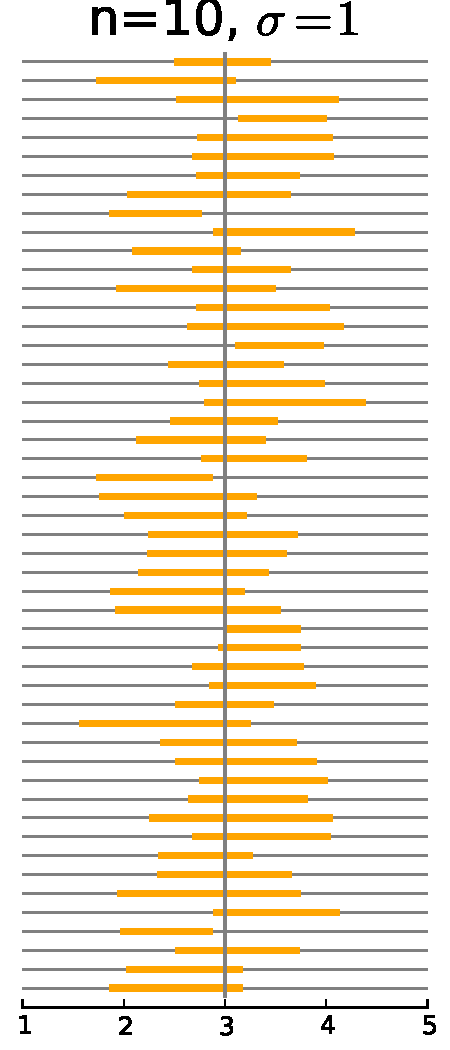
\includegraphics{046-0.pdf}} &
% \scalebox{0.4}{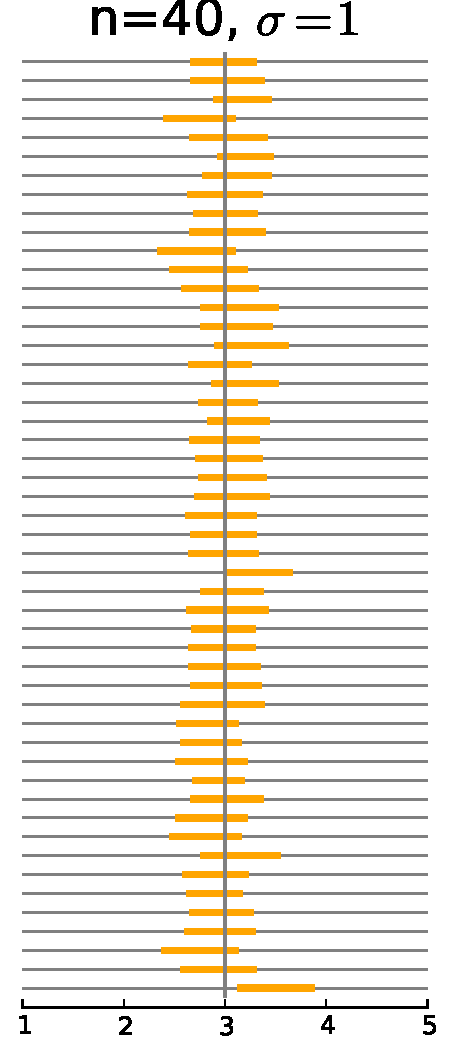
\includegraphics{046-1.pdf}} &
% \scalebox{0.4}{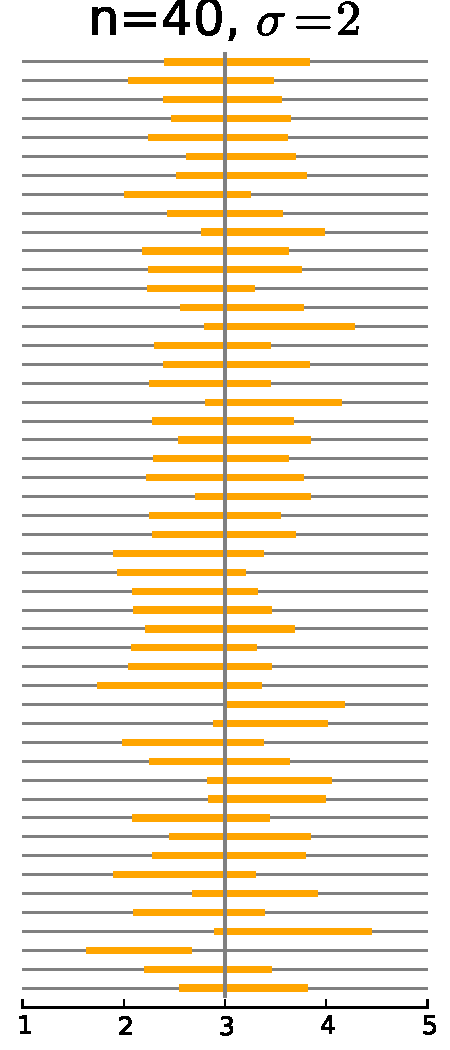
\includegraphics{046-2.pdf}}
% \end{tabular}
% \end{center}

% \end{frame}

% \begin{frame}
% \frametitle{Exercises}

% Suppose we observe a data set containing 8 values:

% \begin{center}
% 8, 4, 5, 4, 6, 3, 4, 5
% \end{center}

% For these values, the sample mean $\bar{X}$ is 4.875.

% \begin{enumerate}

% \item If we are given that the population standard deviation is 1.3,
 % construct a 95\% confidence interval for $EX$.

% \item If we do not know the population standard deviation, but we
 % compute the sample standard deviation as $1.55$, construct a 95\%
 % confidence interval for $EX$.

% \item Suppose we have a data set with 20 values having exactly the
 % same sample mean and standard deviation as the data given above.
 % Construct a 95\% confidence interval for $EX$.

% \end{enumerate}

% \end{frame}

% %%%%%%%%%%%%%%%%%%%%%%%%%%%%%%%%%%%%%%%%%%%%%%%%%%%%%%%%%%%%%%%%%%%%%%%%%%%%%%%%%%
% \begin{frame}
% \frametitle{Solutions}

% \begin{enumerate}

% \item The interval is (4.875-2*1.3/sqrt(8), 4.875+2*1.3/sqrt(8)), or
 % (3.956, 5.794), or 4.875 +/- 0.919.

% \item If the standard deviation is estimated, instead of a multiplier
 % of 2, we should use the 0.975 percentile of a t-distribution with 7
 % degrees of freedom, which is 2.36.  Thus the interval is 4.875 +/-
 % 2.3*1.55/sqrt(8), or 4.875 +/- 1.26.

% \item If the SD is treated as known, as in exercise 1, we would get
 % 4.875 +/- 2*1.3/sqrt(20), or 4.875 +/- 0.58.  If the SD is treated
 % as an estimate, as in number 2, the interval would be 4.875 +/-
 % 2.09*1.55/sqrt(20), or 4.875 +/- 0.72 (note that 2.09 is the 0.975
 % percentile of the t-distribution with 19 degrees of freedom).

% \end{enumerate}

% \end{frame}

% %%%%%%%%%%%%%%%%%%%%%%%%%%%%%%%%%%%%%%%%%%%%%%%%%%%%%%%%%%%%%%%%%%%%%%%%%%%%%%%%%%
% \begin{frame}
% \frametitle{Exercises}

% \begin{enumerate}

% \item Suppose we have two data sets with identical sample means and
 % identical sample variances.  One of the data sets contains twice as
 % many values as the other.  What is the ratio between the lengths of
 % the 95\% confidence intervals for $EX$ in the two data
 % sets?

% \item Supppose we have two data sets with identical sample means and
 % identical sample sizes.  One of the data sets has twice the sample
 % standard deviation of the other.  What is the ratio between the
 % lengths of the 95\% confidence intervals for $EX$ in the two data
 % sets?

% \end{enumerate}

% \end{frame}

% %%%%%%%%%%%%%%%%%%%%%%%%%%%%%%%%%%%%%%%%%%%%%%%%%%%%%%%%%%%%%%%%%%%%%%%%%%%%%%%%%%
% \begin{frame}
% \frametitle{Exercises}

% \begin{enumerate}

% \item The widths of the two intervals will be 4*sigma/sqrt(n) and
 % 4*sigma/sqrt(2*n), so the smaller data set will have a CI that is
 % sqrt(2) times wider than the CI of the larger data set.

% \item The widths of the two intervals are 2*sigma/sqrt(n) and
 % 2*(2*sigma)/sqrt(n).  Thus the data set with the greater standard
 % deviation will have a CI that is two times wider than the CI of the
 % other data set.

% \end{enumerate}

% \end{frame}

% %%%%%%%%%%%%%%%%%%%%%%%%%%%%%%%%%%%%%%%%%%%%%%%%%%%%%%%%%%%
% \begin{frame}[fragile]\frametitle{Graphs of the Various  Z-values}
% \begin{center}
% \includegraphics[width=\linewidth,keepaspectratio]{zval1}
% \end{center}

% \end{frame}

% %%%%%%%%%%%%%%%%%%%%%%%%%%%%%%%%%%%%%%%%%%%%%%%%%%%%%%%%%%%
% \begin{frame}[fragile]\frametitle{Observations}
% \begin{itemize}
% \item For a fixed sample size, the larger the desired confidence, the greater the number of standard deviations that must be used to form the boundary points for the confidence interval.

% \item When the interval becomes wider, the resulting information provides a less precise location of the population mean

% \end{itemize}

% \end{frame}

% %%
% %%%%%%%%%%%%%%%%%%%%%%%%%%%%%%%%%%%%%%%%%%%%%%%%%%%%%%%%%%%%%
% %%\begin{frame}[fragile]\frametitle{T-distribution}
% %%Example: Houehold incomes
% %%\begin{itemize}
% %%\item Sample size = n = 20
% %%\item Average income = 71000
% %%\item Std dev = 2000
% %%\item 95\% confidence interval: $ \mu \pm z_{\alpha/2} \times \sigma/\sqrt{n}$
% %%\item $z_{\alpha/2}$ = 1.96 (as $\alpha = 5$)
% %%\end{itemize}
% %%\begin{center}
% %%\includegraphics[width=0.6\linewidth,keepaspectratio]{tdist1}
% %%\end{center}
% %%\end{frame}


% %%%%%%%%%%%%%%%%%%%%%%%%%%%%%%%%%%%%%%%%%%%%%%%%%%%%%%%%%%%%
% %\begin{frame}[fragile]\frametitle{Estimation Methods}
% %Common approaches
% %\begin{itemize}
% %\item Least squares (LS)
% %\item  Minimize the sum of squares of the deviation
% %\item  Used in linear regression
% %\end{itemize}
% %Maximum likelihood estimation (MLE):  Estimate parameter that is most consistent with the data
% %      Widely used
% %
% %\end{frame}

% %%%%%%%%%%%%%%%%%%%%%%%%%%%%%%%%%%%%%%%%%%%%%%%%%%%%%%%%%%%%%%%%%%%%%%%%%%%%%%%%%%
% \begin{frame}[fragile]\frametitle{}

% \begin{center}
% {\large Estimation}
% \end{center}
% \end{frame}


% %%%%%%%%%%%%%%%%%%%%%%%%%%%%%%%%%%%%%%%%%%%%%%%%%%%%%%%%%%%
% \begin{frame}[fragile]\frametitle{Estimation Theory}

% \begin{itemize}
% \item Many estimates are subjective, that is, a person with experience in the field is utilized to estimate an unknown population value.

% \item The problem with judgment estimates is that their degree of accuracy or inaccuracy cannot be determined.

% \item Even if experts exist, statistics offers estimates with known reliability.

% \end{itemize}

% \end{frame}

% %%%%%%%%%%%%%%%%%%%%%%%%%%%%%%%%%%%%%%%%%%%%%%%%%%%%%%%%%%%
% \begin{frame}[fragile]\frametitle{Estimate/Predict Population Parameter}
% \begin{itemize}
% \item Impossible to measure every member of the population.
% \item So, sample, is measured.
% \item Successful if Sample is ``representative''
% \item Representative: Distributions in Sample-Population similar
% \end{itemize}
% \end{frame}

% %%%%%%%%%%%%%%%%%%%%%%%%%%%%%%%%%%%%%%%%%%%%%%%%%%%%%%%%%%%
% \begin{frame}[fragile]\frametitle{Sampling Types}
% \begin{itemize}
% \item Simple Random Sample (SRS)
% \item Probability Sampling via known distributions
% \item Stratified: SRS with partitions/stratas
% \end{itemize}
% \end{frame}

% %%%%%%%%%%%%%%%%%%%%%%%%%%%%%%%%%%%%%%%%%%%%%%%%%%%%
% %\begin{frame}[fragile] \frametitle{Sampling: Top Sampling}
% %\begin{itemize}
% %\item Select the top s\% of instances from a dataset to create a sample. 
% %\item Top sampling runs a serious risk of introducing bias, the sample will be affected by any ordering of the original dataset 
% %\item Usually avoided
% %\end{itemize}
% %
% %\begin{center}
% %\includegraphics[width=0.6\linewidth,keepaspectratio]{topsample}
% %\end{center}
% %
% %\end{frame}

% %%%%%%%%%%%%%%%%%%%%%%%%%%%%%%%%%%%%%%%%%%%%%%%%%%%
% \begin{frame}[fragile] \frametitle{Sampling: Random Sampling}

% \begin{center}
% \includegraphics[width=0.6\linewidth,keepaspectratio]{randsample}
% \end{center}

% \begin{itemize}
% \item Randomly selects a proportion of s\% of the instances 
% \item Good choice due random nature
% \item Avoids introducing bias 
% \end{itemize}

% \end{frame}


% %%%%%%%%%%%%%%%%%%%%%%%%%%%%%%%%%%%%%%%%%%%%%%%%%%%%%%%%%%
% \begin{frame}[fragile]\frametitle{Stratified Sampling}	
	% \begin{itemize}
	% \item Ensures relative frequencies
	% \item Usage: Skewed proportions amogst classes (chance that they will oget mitted by random sampling)
	% \end{itemize}

% \end{frame}

% %%%%%%%%%%%%%%%%%%%%%%%%%%%%%%%%%%%%%%%%%%%%%%%%%%%%%%%%%%%
% %\begin{frame}[fragile]\frametitle{Other Sampling Forms}	
% %Under-Sampling or Over-Sampling
% %	\begin{itemize}
% %	\item Sample containing different relative frequencies
% %	\item Usage: if we want to have a particular categorical feature be represented equally in the sample, even if that was not the distribution in the original dataset
% %	\end{itemize}
% %
% %\end{frame}


% %%%%%%%%%%%%%%%%%%%%%%%%%%%%%%%%%%%%%%%%%%%%%%%%%%%%%%%%%%%
% \begin{frame}[fragile]\frametitle{Example: Quality Control}
% Point Estimation:
% \begin{itemize}
% \item Point estimates are never perfect.
% \item They have error component, called `` margin of error''.
% \item The error component is expressed as ``confidence interval''.
% \end{itemize}
% %Idea: Take mutiple samples
% \end{frame}


% %%%%%%%%%%%%%%%%%%%%%%%%%%%%%%%%%%%%%%%%%%%%%%%%%%%%%%%%%%%%%%%%%%%%%%%%%%%%%%%%%%
% \begin{frame}[fragile]\frametitle{}
% \begin{center}
% {\Large Example : Ketchup Factory}
% \end{center}
% \end{frame}

% %%%%%%%%%%%%%%%%%%%%%%%%%%%%%%%%%%%%%%%%%%%%%%%%%%%%%%%%%%%
% \begin{frame}[fragile]\frametitle{Example: Sampling Distribution}
% Ketchup Factory:
% \begin{itemize}
% \item Ketchups need to maintain certain viscosity, say , 3200.
% \item At the food processing plant, inspector tests 15 samples.
% \item Point to note: there is no way we can test ALL the Ketchup. 
% \item Must take samples.
% \item From samples, we need to claim viscosity of the whole batch.
% \item As we are not testing ALL, there will be some error. 
% \item Never going to be perfect!!
% \end{itemize}
% \end{frame}

% %%%%%%%%%%%%%%%%%%%%%%%%%%%%%%%%%%%%%%%%%%%%%%%%%%%%%%%%%%%
% \begin{frame}[fragile]\frametitle{Example: Quality Control}
% Sample 1:
% \begin{center}
% \includegraphics[width=0.5\linewidth,keepaspectratio]{qc1}
% \end{center}
% Questions:
% \begin{itemize}
% \item What is the mean of the sample? 
% \item Say, 3210.7
% \item Std dev 117.61
% \end{itemize}
% \end{frame}


% %%%%%%%%%%%%%%%%%%%%%%%%%%%%%%%%%%%%%%%%%%%%%%%%%%%%%%%%%%%
% \begin{frame}[fragile]\frametitle{Example: Quality Control}
% Sample 1:
% \begin{center}
% \includegraphics[width=0.5\linewidth,keepaspectratio]{qc2}
% \end{center}
% \begin{itemize}
% \item Goal was 3200. Sample mean is 3210. Sort of near!!
% \item Is it close enough to pass the batch?
% \item Does it reflect the viscocity `parameter' (ie of population)?
% \end{itemize}
% Plan: Take multiple samples!!!
% \end{frame}

% %%%%%%%%%%%%%%%%%%%%%%%%%%%%%%%%%%%%%%%%%%%%%%%%%%%%%%%%%%%
% \begin{frame}[fragile]\frametitle{Example: Quality Control}

% \begin{center}
% \includegraphics[width=0.5\linewidth,keepaspectratio]{qc4}
% \end{center}
% \begin{itemize}
% \item 9 samples, each of size 15
% \item Calculated their respective means.
% \end{itemize}
% \end{frame}

% %%%%%%%%%%%%%%%%%%%%%%%%%%%%%%%%%%%%%%%%%%%%%%%%%%%%%%%%%%%
% \begin{frame}[fragile]\frametitle{Example: Quality Control}
% \begin{center}
% \includegraphics[width=\linewidth,keepaspectratio]{qc5}
% \end{center}
% \end{frame}

% %%%%%%%%%%%%%%%%%%%%%%%%%%%%%%%%%%%%%%%%%%%%%%%%%%%%%%%%%%%
% \begin{frame}[fragile]\frametitle{Example: Quality Control}
% What is the distribution for sample means?
% \begin{center}
% \includegraphics[width=0.7\linewidth,keepaspectratio]{qc6}
% \end{center}
% Called `Sampling Distribution'.
% Sample distribution is ``Normal''
% \end{frame}

% %%%%%%%%%%%%%%%%%%%%%%%%%%%%%%%%%%%%%%%%%%%%%%%%%%%%%%%%%%%
% \begin{frame}[fragile]\frametitle{Example: Quality Control}
% Sample distribution is ``Normal''
% \begin{itemize}
% \item Expected value (ie Mean) of sample distribution of $\bar{x}$ is population mean $\mu$.
% \item  So, if we take many random samples
% \item Calculate their respective means
% \item Plot them
% \item Find mean of the plot/distribution
% \item Thats the Population Mean!!  Wow!!
% \item We could {\bf infer} parameter of the whole using smaller sets of observations.
% \end{itemize}
% \end{frame}


% %%%%%%%%%%%%%%%%%%%%%%%%%%%%%%%%%%%%%%%%%%%%%%%%%%%%%%%%%%%%%%%%%%%%%%%%%%%%%%%%%%
% \begin{frame}[fragile]\frametitle{}
% \begin{center}
% {\Large Central Limit Theorem}
% \end{center}
% \end{frame}


% %%%%%%%%%%%%%%%%%%%%%%%%%%%%%%%%%%%%%%%%%%%%%%%%%%%%%%%%%%%
% \begin{frame}
% \frametitle{The central limit theorem}

% The normal distribution plays an important role in statistics because
% the average of independent values is usually approximately normal for
% large sample sizes, even if the individual data values are strongly
% non-normal.

% This fact is called the {\bf central limit theorem}.

% \end{frame}

% %%%%%%%%%%%%%%%%%%%%%%%%%%%%%%%%%%%%%%%%%%%%%%%%%%%%%%%%%%%
% \begin{frame}[fragile]\frametitle{Central Limit Theorem}

% {\em When a large number of simple random samples are selected from the population and the mean is calculated for each then the distribution of these sample means will assume the normal probability distribution.  }
 
% \begin{center}
% \includegraphics[width=\linewidth,keepaspectratio]{centrallim}
% \end{center}
% \end{frame}
% %
% %%%%%%%%%%%%%%%%%%%%%%%%%%%%%%%%%%%%%%%%%%%%%%%%%%%%%%%%%%%%%%%%%%%%%%%%
% \begin{frame}[fragile]\frametitle{Sampling a Distribution}
% \begin{columns}
    % \begin{column}[T]{0.6\linewidth}
	% \begin{itemize}
	% \item The original distribution can be anything, Uniform, exponential, etc.
	% \item But once you start taking sample means, the distribution of means is always a Normal Distribution.
	% \end{itemize}

    % \end{column}
    % \begin{column}[T]{0.4\linewidth}
      % \begin{center}
      % \includegraphics[width=\linewidth,keepaspectratio]{statq25}
	  
	  % \includegraphics[width=\linewidth,keepaspectratio]{statq26}
	   
	  	% \end{center}
    % \end{column}

  % \end{columns}
  
% \tiny{(Ref: StatQuest: What is a statistical distribution? - Josh Starmer )}
% \end{frame}


% %%%%%%%%%%%%%%%%%%%%%%%%%%%%%%%%%%%%%%%%%%%%%%%%%%%%%%%%%%%
% \begin{frame}
% \frametitle{The central limit theorem}

% As an illustration of the central limit theorem, suppose $X_1, \ldots,
% X_n$ are values with sample space $\{0,1\}$ and $P(X=1) = 0.8$.  The
% following histograms show the distributions of 10,000 values of
% $\bar{X}$ based on sample sizes $n=5,10,40$ and $80$.

% \begin{center}
% \begin{tabular}{cc}
% \scalebox{0.4}{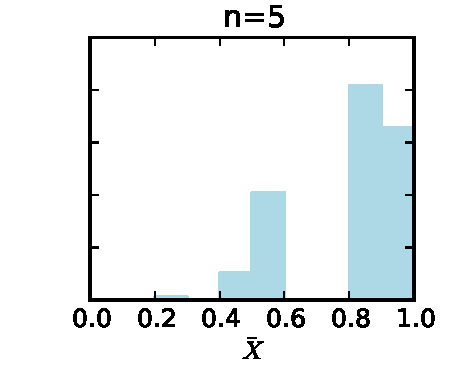
\includegraphics{009_0.pdf}} & 
% \scalebox{0.4}{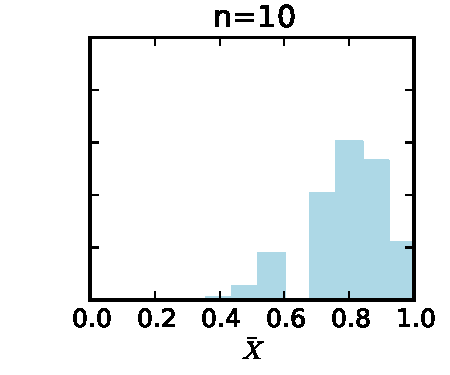
\includegraphics{009_1.pdf}} \\
% \scalebox{0.4}{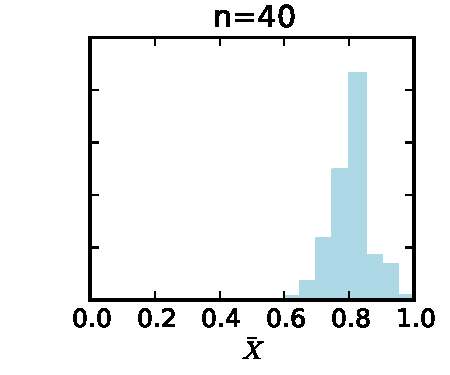
\includegraphics{009_2.pdf}} &
% \scalebox{0.4}{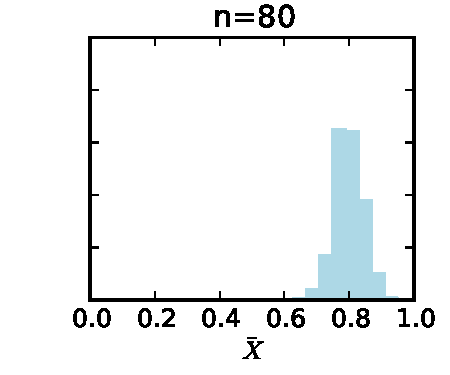
\includegraphics{009_3.pdf}} %http://dept.stat.lsa.umich.edu/~kshedden/Courses/Research_Methods/Slides/009_3.pdf
% \end{tabular}
% \end{center}

% \end{frame}

% %%%%%%%%%%%%%%%%%%%%%%%%%%%%%%%%%%%%%%%%%%%%%%%%%%%%%%%%%%%
% \begin{frame}[fragile]\frametitle{Why Important?}
% \begin{itemize}
% \item Typically, do do not know the distribution present in the population.
% \item Thus, as the Central Limit Theorem, does not care about the distribution, `the distribution of means is always Normal', can be leveraged.
% \item We can then apply t test or others to see similarity between two samples coming from two different populations or batches in Ketchup factory!!!
% \item Just one care: we need to have at-least 30 observations in the sample to be effective (The Rule of Thumb)
% \end{itemize}
% \begin{center}
% \includegraphics[width=0.6\linewidth,keepaspectratio]{statq27}
% \end{center}
% \end{frame}


% %%%%%%%%%%%%%%%%%%%%%%%%%%%%%%%%%%%%%%%%%%%%%%%%%%%%%%%%%%%
% \begin{frame}[fragile]\frametitle{Sampling to find mean of population}
% \begin{itemize}
% \item Intuitive: larger the sample, better the predictive power with Population
% \item: Mathematically: If you plot sample means, that graph's std dev is given as population $\sigma/\sqrt{n}$, where n is the sample size.
% \item So, for large n, std dev goes minimum, narrower.
% \end{itemize}
% \begin{center}
% \includegraphics[width=0.6\linewidth,keepaspectratio]{samplepop}
% \end{center}
% \end{frame}

% %%%%%%%%%%%%%%%%%%%%%%%%%%%%%%%%%%%%%%%%%%%%%%%%%%%

% \begin{frame}[fragile]\frametitle{Example: Quality Control}
% Ketchup Factory:
% \begin{itemize}
% \item For viscosity: Goal is to have population mean as 3200 and std dev as 150
% \item We take 9 samples of 15 measurements each
% \item Past study: mean of the sample distribution is the population mean.
% \end{itemize}
% \begin{center}
% \includegraphics[width=0.8\linewidth,keepaspectratio]{qc5}
% \end{center}
% \end{frame}

% %%%%%%%%%%%%%%%%%%%%%%%%%%%%%%%%%%%%%%%%%%%%%%%%%%%%%%%%%%%
% \begin{frame}[fragile]\frametitle{Example: Quality Control}
% Ketchup Factory:
% \begin{itemize}
% \item We saw mean of sample distribution as population mean.
% \item How much error is there in calculating it.
% \item The formula is $$\sigma_{\bar{x}} = \frac{\sigma}{\sqrt{n}}$$
% \item Represents Std error of mean of the population
% \item In our case $\sigma$ of poulation is given, 150 (if $\sigma$ is unknown, thats another case to look at !!!)
% \item So std error of mean : $$\sigma_{\bar{x}} = \frac{150}{\sqrt{15}} = 38.7$$
% \item As n icreases the error reduces. But not infinetly.
% \end{itemize}

% \end{frame}

% %%%%%%%%%%%%%%%%%%%%%%%%%%%%%%%%%%%%%%%%%%%%%%%%%%%%%%%%%%%
% \begin{frame}[fragile]\frametitle{Example: Quality Control}
% \begin{center}
% \includegraphics[width=0.8\linewidth,keepaspectratio]{qc7}
% \end{center}
% {\bf Std Error of the mean in Population depends only on sample size}
% \end{frame}


% %%%%%%%%%%%%%%%%%%%%%%%%%%%%%%%%%%%%%%%%%%%%%%%%%%%%%%%%%%%%
% %\begin{frame}[fragile]\frametitle{Finding an Estimator}
% %
% %\begin{itemize}
% %\item A perfect estimator would have a mean squared error of zero, but there is no such thing as a perfect estimator.
% %
% %\item Since statistical estimators depend on data which is randomly drawn, they are random variables and cannot always be equal to the true population characteristic.
% %
% %\item The goal is to find an estimator whose average squared error is the smallest.
% %
% %\end{itemize}
% %\end{frame}
% %
% %
% %%%%%%%%%%%%%%%%%%%%%%%%%%%%%%%%%%%%%%%%%%%%%%%%%%%%%%%%%%%%
% %\begin{frame}[fragile]\frametitle{Restricting Estimators}
% %There are an infinite number of possible estimators and without restricting the kinds of estimators that will be considered, very little progress can be made.
% %
% %\end{frame}
% %
% %
% %%%%%%%%%%%%%%%%%%%%%%%%%%%%%%%%%%%%%%%%%%%%%%%%%%%%%%%%%%%%
% %\begin{frame}[fragile]\frametitle{Unbiasedness}
% %\begin{itemize}
% %\item On desirable restriction is unbiasedness.
% %
% %\item To be an unbiased estimator, the expected value of the estimator must be equal to the parameter that is being estimated.
% %
% %\item For example,  $\bar{x}$  is an unbiased estimator of the population mean since
% %$$ E(\bar{x}) = \mu$$
% %
% %\end{itemize}
% %
% %\end{frame}
% %

% %%%%%%%%%%%%%%%%%%%%%%%%%%%%%%%%%%%%%%%%%%%%%%%%%%%%%%%%%%%
% \begin{frame}[fragile]\frametitle{Example: Quality Control}
% \begin{itemize}
% %\item The sampling distrubution graph is a bit coarse.
% %\item If we had taken MANY samples, the population mean would be MORE accurate.
% %\item But then, whats the point?
% \item Need some estimation of how good the current estimation of population mean is, with only few samples.
% \item For this, we find Interval Estimate of the population mean.
% \end{itemize}
% \end{frame}
% %
% %%%%%%%%%%%%%%%%%%%%%%%%%%%%%%%%%%%%%%%%%%%%%%%%%%%%%%%%%%%%%%%%%%%%%%%%%%%%%%%%%%
% \begin{frame}[fragile]\frametitle{}
% \begin{center}
% {\Large Interval Estimate}
% \end{center}
% \end{frame}


% %%%%%%%%%%%%%%%%%%%%%%%%%%%%%%%%%%%%%%%%%%%%%%%%%%%%%%%%%%%
% \begin{frame}[fragile]\frametitle{Example: Quality Control}
% Interval Estimate:
% \begin{itemize}
% \item Interval Estimate will be influenced by Sample size and the degree of ``confidence'' we wish to have.
% \item E.g. which is better, if we have 5 measuremens in a sample or 15?
% \item E.g. which is better, if we allow 3\% error or 10\% error in our estimates?
% \end{itemize}
% \end{frame}


% %%%%%%%%%%%%%%%%%%%%%%%%%%%%%%%%%%%%%%%%%%%%%%%%%%%%%%%%%%%
% \begin{frame}[fragile]\frametitle{Constructing an Interval estimator}
% An interval estimator is made by developing an upper and a lower boundary for an interval that will hopefully contain the population parameter.

% \end{frame}

% %%%%%%%%%%%%%%%%%%%%%%%%%%%%%%%%%%%%%%%%%%%%%%%%%%%%%%%%%%%%
% %\begin{frame}[fragile]\frametitle{Constructing an Interval estimator}
% %\begin{itemize}
% %\item However, this particular interval estimator would not contain any useful information about the location of the population parameter.
% %
% %\item In interval estimation, the smaller the interval for a given amount of confidence, the better.
% %
% %
% %\end{itemize}
% %
% %\end{frame}

% %%%%%%%%%%%%%%%%%%%%%%%%%%%%%%%%%%%%%%%%%%%%%%%%%%%%%%%%%%%%
% %\begin{frame}[fragile]\frametitle{Estimation: Point vs. Interval}
% %\begin{itemize}
% %\item Point estimation
% % Use one single number as the best estimator
% %for a specific population parameter
% % ``Point estimator''
% % E.g. estimator for mean=15
% %\item  Interval estimation, ``Confidence Interval''
% % use a range of numbers within which the
% %    parameter is believed to fall (lower bound,
% %    upper bound)
% % e.g. (10, 20)
% %
% %\end{itemize}
% %
% %\end{frame}

% %%%%%%%%%%%%%%%%%%%%%%%%%%%%%%%%%%%%%%%%%%%%%%%%%%%%%%%%%%%
% \begin{frame}[fragile]\frametitle{Estimation: Example}
% \begin{itemize}
% \item The sampling distribution can be used to develop an interval estimator.

% \item For the standard normal random variable,
% $$P(-2.17 < z < 2.17) = .97 $$

% \end{itemize}

% \end{frame}

% %%%%%%%%%%%%%%%%%%%%%%%%%%%%%%%%%%%%%%%%%%%%%%%%%%%%%%%%%%%
% \begin{frame}[fragile]\frametitle{Estimation: Example}
% \begin{itemize}
% \item Since $\bar{x}$ can be transformed in the standard normal random variable by using the z-transform,
% $$ z = \frac{\bar{x} - \mu}{\sigma_{\bar{x}}}$$

% \item then by substitution,

% $$P(-2.17 < \frac{\bar{x} - \mu}{\sigma_{\bar{x}}} < 2.17) = .97 $$

% \item and with some algebraic manipulation we obtain
% $$P(\bar{x} -2.17 \sigma_{\bar{x}} <  \mu <\bar{x} + 2.17 \sigma_{\bar{x}}) = .97 $$

% \end{itemize}

% \end{frame}

% %%%%%%%%%%%%%%%%%%%%%%%%%%%%%%%%%%%%%%%%%%%%%%%%%%%%%%%%%%%%
% %\begin{frame}[fragile]\frametitle{Estimation: Example}
% %\begin{itemize}
% %\item Since $\bar{x}$ can be transformed in the standard normal random variable by using the z-transform,
% %$$ z = \frac{\bar{x} - \mu}{\sigma_{\bar{x}}}$$
% %
% %\item then by substitution,
% %
% %$$P(-2.17 < \frac{\bar{x} - \mu}{\sigma_{\bar{x}}} < 2.17) = .97 $$
% %
% %\item and with some algebraic manipulation we obtain
% %$$P(\bar{x} -2.17 \sigma_{\bar{x}} <  \mu <\bar{x} + 2.17 \sigma_{\bar{x}}) = .97 $$
% %
% %\end{itemize}
% %
% %\end{frame}

% %%%%%%%%%%%%%%%%%%%%%%%%%%%%%%%%%%%%%%%%%%%%%%%%%%%%%%%%%%%
% \begin{frame}[fragile]\frametitle{Estimation: Example}
% $$P(\bar{x} -2.17 \sigma_{\bar{x}} <  \mu <\bar{x} + 2.17 \sigma_{\bar{x}}) = .97 $$
% \begin{itemize}
% \item The expression suggests a specific form for the interval. 

% \item The population mean will fall within the interval
% $$ \bar{x} \pm 2.17 \sigma_{\bar{x}}$$ 97\% of times
% \end{itemize}

% \end{frame}


% %%%%%%%%%%%%%%%%%%%%%%%%%%%%%%%%%%%%%%%%%%%%%%%%%%%%%%%%%%%
% \begin{frame}[fragile]\frametitle{Estimation: Example}

% \begin{itemize}
% %\item After the sample is selected, the sample mean is no longer a random variable.
% %
% %\item $\bar{x}$ is a random variable, but    $\bar{x} = 33.2$  is the sample mean for a particular sample.

% \item 
% Suppose a sample has been drawn from a population with a standard deviation of 200, and the following characteristics have been observed:
% $n = 100$, and $\bar{x} = 150$.
% $$ \sigma_{\bar{x}} = \frac{\sigma}{\sqrt{n}} = \frac{200}{\sqrt{100}}$$
% \item Resulting interval = $150 \pm 2.17 (200/10)$ ie 106.6 to 193.4
% \end{itemize}

% \end{frame}


% %%%%%%%%%%%%%%%%%%%%%%%%%%%%%%%%%%%%%%%%%%%%%%%%%%%%%%%%%%%%
% %\begin{frame}[fragile]\frametitle{Estimation: Example}
% %
% %\begin{itemize}
% %\item Even though the interval is calculated using a technique that captures the population mean 97\% of the time, it would not be appropriate, from a relative frequency point of view, to state that
% %$$P(106.6 < \mu < 193.4) = .97 $$
% %\item Since the population mean is an unknown but constant quantity. Either it will always be inside the interval or will be outside the interval due to only 97\% confidence
% %\item Hence, the term confidence interval is used to describe the method of construction rather than a particular interval.
% %
% %\end{itemize}
% %\end{frame}




